\section{Experimental setup}
\label{sec:setup}

The official chapter-level evaluation uses the 30 videos listed in
\texttt{data/manifest.jsonl} and the creator-provided YouTube chapter
boundaries in \texttt{data/gt/}. Metrics were computed with the project
implementation in \texttt{src/lecseg/metrics.py}. Unless stated otherwise,
all values are macro averages over the 30 videos. Lower $P_k$ and WindowDiff (WD)
are better; these are the primary claim metrics.
Boundary Similarity (BS) and tolerance-$F_1$ are secondary diagnostics;
higher is better but neither drives method ranking.
See Section~\ref{sec:secondary_metrics} for the rationale.

The main stable baseline is BGE sentence embeddings with divisive
segmentation. The best joint $P_k$/WindowDiff run combines BGE/E5-style
cross-model boundary scoring with conservative minimum-length postprocessing
and the alignment-audited reference mapping
(\texttt{cross\_e5\_frac70\_minlen11\_\_align\_contains\_before} in
\texttt{results/eval\_alignment\_sweep.json}). A separate leave-one-video-out
method selector improves mean $P_k$, WD, and boundary-hit metrics, though the
$P_k$/WD gains over the cross-model method are not significant.

\section{Official result and claim boundary}
\label{sec:official_claim}

The official deployable claim of this thesis is deliberately conservative. The
safest single global method is the cross-model conservative run because it
significantly improves $P_k$ and WindowDiff over the BGE-divisive baseline. The
balanced selector is reported as the best mean local operating point and as
evidence that method-choice information is useful, but it is not claimed as a
fully domain-general replacement: its $P_k$/WD gains over the cross-model method
are not statistically significant, and its leave-domain-out result is weaker.
Oracle results are used only to diagnose the remaining candidate-selection gap.

\begin{table}[t]
  \centering
  \caption{Claim--evidence--caveat audit for the final thesis narrative.}
  \label{tab:claim_evidence_caveat}
  \resizebox{\linewidth}{!}{%
  \begin{tabular}{p{0.27\linewidth}p{0.33\linewidth}p{0.33\linewidth}}
    \toprule
    Claim & Evidence & Caveat \\
    \midrule
    \dataset{} is a real low-resource lecture benchmark &
    30 videos, 32.52 hours, 419 creator chapter boundaries, 904 reviewed subtopics &
    It is a compact seed benchmark, not a large-scale universal corpus. \\
    Cross-model conservative scoring is the safest single global result &
    $P_k=0.3713$, WD $=0.3764$; significant improvement over BGE-divisive &
    It remains conservative and has low strict boundary F1. \\
    Balanced selector gives the best mean local operating point &
    $P_k=0.3588$, WD $=0.3739$, F1@2 $=0.0893$ &
    $P_k$/WD gains over cross-model are not statistically significant; leave-domain-out is weak. \\
    CLIP is the most promising non-text signal &
    CLIP+text reaches $P_k=0.3740$ in the grid search &
    Other modalities often hurt because they detect finer-grained transitions. \\
    LLM refinement is implemented &
    \texttt{llm\_refine.py}; LLM zero-shot diagnostic result exists &
    Full before/after LLM boundary improvement is not established; do not make it the headline claim. \\
    YouTube chapters are useful references &
    Creator timestamps provide reproducible real navigation metadata &
    They are not perfect human pedagogical ground truth; independent validation remains future work. \\
    \bottomrule
  \end{tabular}
  }
\end{table}


\section{Dataset and annotation status}
\label{sec:dataset_status}

\dataset{} contains 30 lectures, 32.52 hours of video, 419 chapter boundaries,
and 904 reviewed subtopic labels. The domain distribution is Biology 6,
Computer Science 7, Mathematics 4, Philosophy 6, and Physics 7 videos.
The current manifest is cross-domain but not perfectly balanced.

\begin{table}[t]
  \centering
  \caption{Inter-annotator agreement at zero-tolerance (exact sentence match),
    measured between two independent human annotators.
    The chapter-level $F_1=1.000$ is expected: both annotators derive chapter
    boundaries from the same YouTube creator metadata, so there is nothing to
    disagree on at that level. The subtopic $\kappa=0.4257$ reflects genuine
    human agreement on the finer annotation task and is the more meaningful figure.}
  \label{tab:iaa}
  \begin{tabular}{lcc}
    \toprule
    Level & Cohen's $\kappa$ & Boundary $F_1$ \\
    \midrule
    Chapter & 0.5351 & 1.0000 \\
    Subtopic & 0.4257 & 0.7793 \\
    \bottomrule
  \end{tabular}
\end{table}

\section{Main results}
\label{sec:main}

\begin{table}[t]
\centering
\small
\caption{Current LECSEG result variants and diagnostic upper bound.}
\label{tab:lecseg_result_variants}
\begin{tabularx}{\linewidth}{lrrrrX}
\toprule
Method & Pk & WD & BS & F1@2 & Role \\
\midrule
BGE-divisive baseline & 0.3884 & 0.3956 & 0.1292 & 0.0878 & Strong implemented baseline \\
Cross-model conservative & 0.3713 & 0.3764 & 0.0362 & 0.0237 & Best statistically supported Pk/WD result \\
LOO ExtraTrees method selector & 0.3588 & 0.3739 & 0.0757 & 0.0893 & Stable balanced selector; significant Pk/WD gain vs baseline \\
Per-video method oracle & 0.2980 & 0.3280 & 0.1366 & 0.1676 & Diagnostic upper bound, not deployable \\
\bottomrule
\end{tabularx}
\end{table}

Table~\ref{tab:lecseg_result_variants} shows three consistent patterns.
The BGE-divisive baseline is substantially stronger than the classical and
neural alternatives under $P_k$ and WD, confirming that dense embeddings
are the right foundation for this task. Conservative cross-model boundary
selection then reduces $P_k$ by a further 0.0171 absolute, which is the best
statistically supported joint $P_k$/WD result in the evaluation.
The method selector reaches the best mean $P_k$ and produces markedly higher
F1@2, though its $P_k$/WD gains over the cross-model method do not individually
reach significance.

\begin{figure}[t]
  \centering
  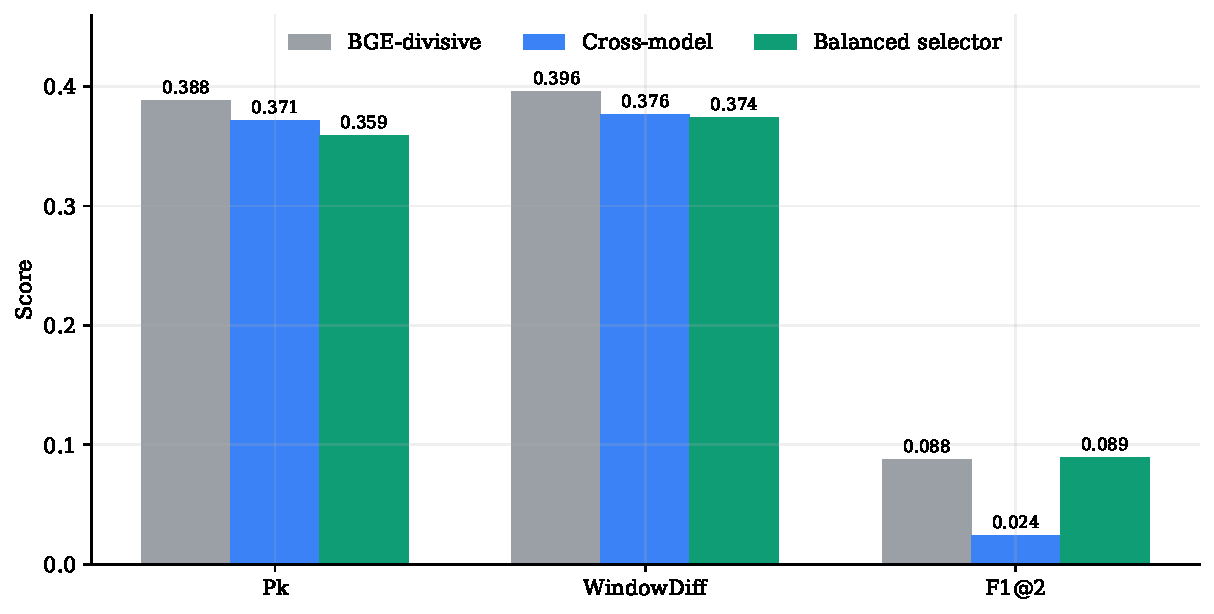
\includegraphics[width=\linewidth]{figures/fig_final_results.pdf}
  \caption{Primary LECSEG-30 operating points. Lower is better for $P_k$ and
  WindowDiff; higher is better for F1@2. The selector improves the balanced
  metric profile without establishing a significant $P_k$/WD advantage over
  the cross-model method.}
  \label{fig:final_results}
\end{figure}

\begin{table}[t]
\centering
\caption{Paired Wilcoxon significance tests for key LECSEG comparisons.}
\label{tab:lecseg_significance}
\begin{tabular}{p{0.30\linewidth}lrrlp{0.09\linewidth}}
\toprule
Comparison & Metric & Delta & p & Significant & Wins \\
\midrule
Cross-model vs BGE baseline & pk & -0.0171 & 0.0064 & yes & 22/30 \\
Cross-model vs BGE baseline & wd & -0.0193 & 0.0001 & yes & 26/30 \\
Cross-model vs BGE baseline & boundary\_similarity & -0.0930 & 0.0074 & yes & 4/30 \\
Cross-model vs BGE baseline & f1\_tol2 & -0.0641 & 0.0090 & yes & 4/30 \\
Selector vs cross-model & pk & -0.0126 & 0.3560 & no & 9/30 \\
Selector vs cross-model & wd & -0.0025 & 0.9039 & no & 7/30 \\
Selector vs cross-model & boundary\_similarity & 0.0395 & 0.0076 & yes & 10/30 \\
Selector vs cross-model & f1\_tol2 & 0.0656 & 0.0076 & yes & 10/30 \\
Selector vs BGE baseline & pk & -0.0296 & 0.0252 & yes & 19/30 \\
Selector vs BGE baseline & wd & -0.0217 & 0.0238 & yes & 23/30 \\
Selector vs BGE baseline & boundary\_similarity & -0.0534 & 0.1541 & no & 8/30 \\
Selector vs BGE baseline & f1\_tol2 & 0.0015 & 0.9170 & no & 9/30 \\
\bottomrule
\end{tabular}
\end{table}

Table~\ref{tab:lecseg_significance} separates mean improvements from
statistically supported claims. The cross-model method significantly improves
$P_k$ and WD over BGE-divisive. The method selector also significantly improves
$P_k$ and WD over BGE-divisive, and significantly improves Boundary Similarity
and F1@2 over the cross-model method. Its $P_k$/WD gains over the cross-model
method are not significant, so it is best read as a stronger
operating-point experiment rather than a conclusive replacement.

\begin{table}[t]
\centering
\small
\caption{Selector and ranker operating points on LECSEG-30.}
\label{tab:selector_operating_points}
\begin{tabularx}{\linewidth}{lrrrrX}
\toprule
Operating point & Pk & WD & BS & F1@2 & Role \\
\midrule
BGE-divisive baseline & 0.3884 & 0.3956 & 0.1292 & 0.0878 & Stable implemented baseline \\
Cross-model conservative & 0.3713 & 0.3764 & 0.0362 & 0.0237 & Best single global Pk/WD method \\
Pk-ranked selector & 0.3739 & 0.3867 & 0.0654 & 0.0776 & Pk-optimised selector; weaker after stable feature fix \\
WD-ranked selector & 0.3703 & 0.3823 & 0.0584 & 0.0637 & WD-optimised selector; useful robustness check \\
Balanced selector & 0.3588 & 0.3739 & 0.0757 & 0.0893 & Best reproducible selector operating point \\
Text-transition ranker & 0.3937 & 0.4154 & 0.1163 & 0.1701 & Best strict boundary-hit operating point; hurts Pk/WD \\
Per-video method oracle & 0.2980 & 0.3280 & 0.1366 & 0.1676 & Diagnostic upper bound, not deployable \\
\bottomrule
\end{tabularx}
\end{table}

Table~\ref{tab:selector_operating_points} explains why the balanced selector is
used as the selector result. Ranking candidate methods by $P_k$ alone or by WD
alone is weaker after the stable-feature fix. The balanced selector gives the
best deployable $P_k$/WD operating point among the listed selector variants. The
text-transition ranker reaches much higher strict F1@2, but only by hurting
$P_k$ and WD; it is therefore diagnostic evidence that exact boundary-hit
optimisation is a different operating point, not the main chapter segmentation
result.

\begin{table}[t]
\centering
\small
\caption{Balanced selector robustness across candidate method-pool sizes.}
\label{tab:selector_robustness}
\begin{tabular}{lrrrrr}
\toprule
Setting & top-$k$ & Pk & WD & BS & F1@2 \\
\midrule
k30 & 30 & 0.3729 & 0.3780 & 0.0317 & 0.0226 \\
k50 & 50 & 0.3634 & 0.3760 & 0.0495 & 0.0608 \\
k80 & 80 & 0.3588 & 0.3739 & 0.0757 & 0.0893 \\
k120 & 120 & 0.3716 & 0.3852 & 0.0774 & 0.0929 \\
\bottomrule
\end{tabular}
\end{table}

Table~\ref{tab:selector_robustness} checks that the selector result is not
an arbitrary single setting. The balanced selector improves as the
candidate method pool grows from 30 to 80 methods, then degrades at 120 methods.
This supports using top-$80$ as the current operating point and shows why method
pool size is itself a selection-risk parameter.

\begin{table}[t]
\centering
\small
\caption{Domain-level Pk/WD for baseline, cross-model, and balanced selector.}
\label{tab:domain_performance}
\resizebox{\linewidth}{!}{%
\begin{tabular}{lrrrrrrrr}
\toprule
Domain & Videos & Chapters & Base Pk & Cross Pk & Sel. Pk & Base WD & Cross WD & Sel. WD \\
\midrule
Biology & 6 & 94 & 0.4218 & 0.3968 & 0.3976 & 0.4292 & 0.4008 & 0.4152 \\
CS & 7 & 98 & 0.3409 & 0.3295 & 0.3314 & 0.3439 & 0.3336 & 0.3357 \\
Math & 4 & 55 & 0.3724 & 0.3792 & 0.4014 & 0.3850 & 0.3873 & 0.4367 \\
Philosophy & 6 & 122 & 0.4415 & 0.3948 & 0.3753 & 0.4544 & 0.4057 & 0.3893 \\
Physics & 7 & 50 & 0.3710 & 0.3667 & 0.3144 & 0.3742 & 0.3667 & 0.3276 \\
\bottomrule
\end{tabular}
}
\end{table}


Table~\ref{tab:domain_performance} shows that the selector improvement is not
uniform across subjects. Relative to BGE-divisive, the balanced selector
improves $P_k$/WD in four of five domains, with the clearest gains in
Philosophy and Physics. Mathematics is the main failure case: the selector
worsens both $P_k$ and WD there, suggesting that the current method selector
does not have enough domain-specific evidence to avoid poor choices on the
smallest domain split.

\begin{figure}[t]
  \centering
  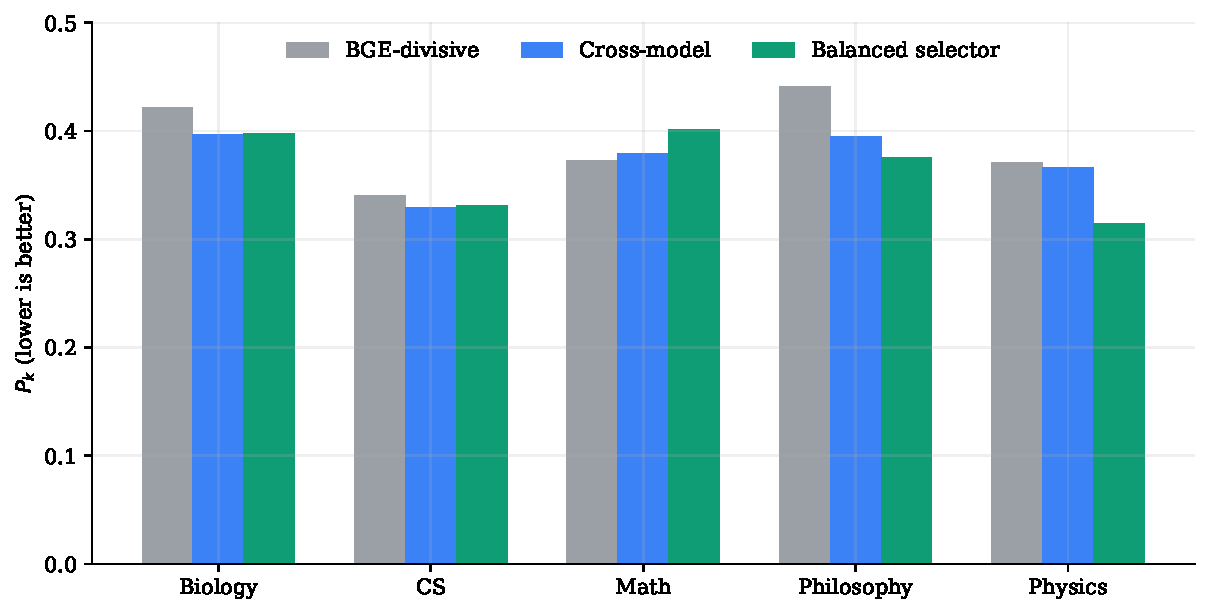
\includegraphics[width=\linewidth]{figures/fig_domain_performance.pdf}
  \caption{Domain-level $P_k$ comparison. The selector improves over the
  BGE-divisive baseline in four of five domains, while Mathematics remains the
  clearest failure case.}
  \label{fig:domain_performance}
\end{figure}

\begin{table}[t]
\centering
\small
\caption{Largest balanced-selector per-video Pk changes relative to the cross-model method.}
\label{tab:selector_choice_audit}
\begin{tabular}{llrrrr}
\toprule
Video & Domain & $\Delta P_k$ & Sel. Pk & Cross Pk & $\Delta$F1@2 \\
\midrule
Hy7ou5R\_vjE & Physics & -0.1542 & 0.1375 & 0.2917 & 0.0000 \\
YdOXS\_9\_P4U & Physics & -0.1261 & 0.3009 & 0.4270 & 0.0000 \\
NK-BxowMIfg & Physics & -0.0861 & 0.3583 & 0.4444 & 0.0000 \\
j0wJBEZdwLs & Math & 0.0754 & 0.4559 & 0.3805 & 0.0000 \\
oOya3cFmAMc & Biology & 0.0529 & 0.4835 & 0.4306 & 0.1667 \\
D8RRq3TbtHU & CS & 0.0119 & 0.3638 & 0.3519 & 0.0000 \\
\bottomrule
\end{tabular}
\end{table}

Table~\ref{tab:selector_choice_audit} audits the selector at the individual
video level. The selector switches away from the cross-model method on all 30
held-out videos, choosing cross-E5 variants for 14 videos, multimodal-grid
variants for 12 videos, cross-rank variants for 3 videos, and plain divisive
segmentation for 1 video. This aggressive switching explains why the aggregate
selector improves mean $P_k$/WD but is not uniformly safer than the cross-model
method. The largest gains are on Physics videos where multimodal-grid variants
substantially reduce $P_k$; the largest regressions occur on Math and Biology
videos where the same family over-selects weaker operating points.

\begin{table}[t]
  \centering
  \caption{Same-dataset comparison on LECSEG-30. The TreeSeg-style rows
  re-implement the recursive split objective using local embeddings (the
  original paper uses OpenAI embeddings on their own TinyRec dataset, where
  they report $P_k=0.367$; that number is \emph{not} directly comparable here
  because the datasets differ). Lower is better for $P_k$/WD; higher for F1@2.}
  \label{tab:same_dataset_comparison}
  \small
  \resizebox{\linewidth}{!}{%
  \begin{tabular}{lrrrl}
    \toprule
    Method & $P_k\downarrow$ & WD$\downarrow$ & F1@2$\uparrow$ & Interpretation \\
    \midrule
    Balanced LOO selector & 0.3588 & 0.3739 & 0.0893 & Official LECSEG best \\
    Cross-model conservative & 0.3713 & 0.3764 & 0.0237 & Best single global method \\
    TreeSeg-style (MPNet, LECSEG-30) & 0.4320 & 0.4673 & 0.1733 & Higher F1, worse $P_k$/WD \\
    TreeSeg-style (E5-large, LECSEG-30) & 0.4322 & 0.4654 & 0.1576 & Same-dataset comparator \\
    TreeSeg-style (BGE-large, LECSEG-30) & 0.4399 & 0.4780 & 0.1643 & Same-dataset comparator \\
    \midrule
    TreeSeg paper (on TinyRec)\textsuperscript{$\dagger$} & 0.367 & --- & --- & Different dataset; indicative only \\
    \bottomrule
  \end{tabular}%
  }
  \vspace{0.3em}
  \small\textsuperscript{$\dagger$}~Gklezakos et al.\ (2024), arxiv:2407.12028. Evaluated on 21 self-recorded lectures (TinyRec), not LECSEG-30.
\end{table}


Table~\ref{tab:same_dataset_comparison} addresses a common comparison
objection by evaluating a TreeSeg-style public split objective on the same
\dataset{} benchmark with local LECSEG embeddings. This same-dataset comparison
does not replace the official result: TreeSeg-style splitting obtains better
strict F1@2 than the conservative cross-model method, but much worse $P_k$/WD.
The result clarifies the operating-point tradeoff. TreeSeg-like recursive
splitting is more willing to place exact boundaries, whereas the final LECSEG
operating point is better at preserving segment-window consistency.

\begin{table}[t]
\centering
\small
\caption{Leave-one-domain-out selector diagnostic.}
\label{tab:selector_leave_domain_out}
\begin{tabular}{lrrrr}
\toprule
Method & Pk & WD & BS & F1@2 \\
\midrule
BGE-divisive baseline & 0.3884 & 0.3956 & 0.1292 & 0.0878 \\
Cross-model conservative & 0.3713 & 0.3764 & 0.0362 & 0.0237 \\
Leave-domain-out selector & 0.4012 & 0.4103 & 0.0465 & 0.0498 \\
\bottomrule
\end{tabular}
\end{table}

Table~\ref{tab:selector_leave_domain_out} applies a stricter diagnostic:
training excludes the entire held-out academic domain. Under this setting the
selector degrades to $P_k=0.4012$ and WD $=0.4103$, worse than both
BGE-divisive and the cross-model method. This negative result is important for
interpretation: the leave-one-video-out improvement relies on having related
domains in the training fold. The current selector should therefore be treated
as a low-resource benchmark operating point, not a domain-general deployment model.

\section{Deployment-style boundary diagnostics}
\label{sec:modern_metrics}

Strict F1@2 is a useful exact-boundary diagnostic, but it does not tell the
whole story. A lecture navigation system may still be useful when a boundary
is near the correct region but not within two sentences. To expose this
tradeoff, we add a diagnostic evaluation with wider sentence tolerances,
time tolerances, segment-overlap scoring, and boundary-count error. These
figures are not a replacement for the official alignment-sweep and selector
results; they are a deployment-style interpretation layer generated by
\texttt{scripts/evaluate\_modern\_metrics.py}.

\begin{table}[t]
\centering
\caption{Modern boundary and segment metrics for defended operating points. Lower Pk, WD, and count error are better; higher F1 and tIoU are better.}
\label{tab:modern_metrics}
\resizebox{\linewidth}{!}{%
\begin{tabular}{lrrrrrrrr}
\toprule
Method & Pk & WD & F1@2 & F1@5 & F1@10 & F1@30s & tIoU & Count Err. \\
\midrule
BGE-divisive baseline & 0.4197 & 0.4252 & 0.0394 & 0.0404 & 0.0517 & 0.0448 & 0.0806 & 0.00 \\
Cross-model conservative & 0.4071 & 0.4124 & 0.0273 & 0.0476 & 0.0756 & 0.0655 & 0.3810 & 11.47 \\
Conservative smoothed BGE & 0.4158 & 0.4222 & 0.0464 & 0.0621 & 0.0728 & 0.0652 & 0.1165 & 4.17 \\
Two-stage predictor & 0.4620 & 0.5058 & 0.0882 & 0.1285 & 0.1776 & 0.1635 & 0.2981 & 0.00 \\
Hierarchical segmenter & 0.4351 & 0.4419 & 0.0280 & 0.0402 & 0.0835 & 0.0611 & 0.3456 & 9.70 \\
\bottomrule
\end{tabular}
}
\end{table}


\begin{figure}[t]
  \centering
  
\includegraphics[width=\linewidth]{figures/modern_metrics_structure_vs_f1.pdf}
  \caption{Diagnostic comparison between broad structure quality and strict
  boundary-hit metrics. Lower $P_k$ is better; higher F1 is better. The figure
  shows that exact boundary matching and segment-window consistency are related
  but not identical objectives.}
  \label{fig:modern_structure_f1}
\end{figure}

\begin{figure}[t]
  \centering
  
\includegraphics[width=\linewidth]{figures/modern_metrics_boundary_count_error.pdf}
  \caption{Mean boundary count error. Negative values mean a method predicts
  fewer boundaries than the creator reference; positive values mean
  over-segmentation. Count behaviour explains why conservative methods can score
  well on $P_k$/WD while remaining weak on strict F1.}
  \label{fig:boundary_count_error}
\end{figure}

\begin{figure}[t]
  \centering
  
\includegraphics[width=\linewidth]{figures/modern_metrics_time_segment.pdf}
  \caption{Video-oriented relaxed metrics: F1 within 30 seconds and mean best
  temporal segment overlap. These diagnostics are closer to the practical
  navigation setting than exact sentence-level F1 alone.}
  \label{fig:modern_time_segment}
\end{figure}

Table~\ref{tab:modern_metrics} shows why the low strict F1 must be read
carefully. The cross-model method has the best diagnostic $P_k$/WD among the
rerun operating points and the strongest segment-overlap score, but it is very
conservative and under-predicts boundaries. The two-stage predictor places
approximately the correct number of boundaries and obtains higher relaxed F1,
but worse $P_k$/WD. Exact boundary hitting and broad segment structure are
different objectives; a deployable future system would need to optimise both.

\section{Ablation and diagnostic findings}
\label{sec:ablations}

\begin{table}[t]
  \centering
  \caption{Selected ablations and diagnostics.}
  \label{tab:ablation}
  \resizebox{\linewidth}{!}{%
  \begin{tabular}{lrrl}
    \toprule
    Variant & $P_k\downarrow$ & WD$\downarrow$ & Interpretation \\
    \midrule
    BGE + divisive & 0.3884 & 0.3956 & Stable text-only baseline \\
    Hierarchical & 0.4118 & 0.4206 & Useful representation, weaker chapter Pk \\
    TwoStage + prosody & 0.4333 & 0.4970 & Higher F1, worse Pk/WD \\
    BERT-wiki zero-shot & 0.4932 & 0.5397 & Poor domain transfer \\
    Discourse markers (forced boundaries) & 0.4615 & 0.5221 & Over-segments at subtopic level \\
    BERTopic topic-shift & 0.5632 & 0.6984 & Finds subtopics, not chapters \\
    GPT-2 perplexity (200 sent.\ cap) & 0.4182 & 0.4316 & Language surprise detects subtopic shifts \\
    LLM zero-shot Llama-3.1-8B (3 videos) & 0.4056 & 0.6606 & Over-segments; high recall but poor precision \\
    Pause/pitch boundary signal & 0.4174 & 0.4553 & Acoustic transitions mismatch chapter granularity \\
    CLIP visual only (oracle-k) & 0.3958 & -- & Surprisingly strong visual signal \\
    CLIP + text fusion (best grid) & 0.3740 & 0.4085 & Beats BGE-divisive; near cross-model \\
    Boundary classifier LOOCV & 0.5803 & 0.9933 & Over-predicts boundaries \\
    Text-transition ranker & 0.3868 & $\approx$0.40 & Higher F1, weaker than official Pk/WD \\
    Oracle-k divisive & 0.4237 & -- & Segment count is not the bottleneck \\
    \bottomrule
  \end{tabular}
  }
\end{table}

\begin{table}[t]
  \centering
  \caption{Status of LLM and multimodal claims.}
  \label{tab:llm_fusion_status}
  \resizebox{\linewidth}{!}{%
  \begin{tabular}{p{0.24\linewidth}rrp{0.42\linewidth}}
    \toprule
    Component & $P_k$ & WD & Interpretation \\
    \midrule
    BGE-divisive text baseline & 0.3884 & 0.3956 &
    Stable chapter-level anchor. \\
    CLIP+text best grid & 0.3740 & 0.4085 &
    Visual slide/scene signal helps $P_k$ and is the strongest non-text cue, but WD is weaker than cross-model text. \\
    Pause/pitch signal & 0.4174 & 0.4553 &
    Acoustic transitions detect finer rhetorical or subtopic shifts and hurt chapter-level segmentation. \\
    BERTopic topic-shift & 0.5632 & 0.6984 &
    Topic modeling over-segments relative to creator chapter granularity. \\
    LLM zero-shot (3 videos) & 0.4056 & 0.6606 &
    Over-segments strongly; diagnostic only, not a final segmentation improvement. \\
    LLM candidate verifier (partial) & -- & -- &
    Implemented and partially evaluated, but no full-scale final metric gain is established. \\
    \bottomrule
  \end{tabular}
  }
\end{table}


The negative results are as informative as the positive ones.
Discourse markers ($P_k=0.4615$), BERTopic ($P_k=0.5632$), GPT-2 perplexity
($P_k=0.4182$), and acoustic transitions ($P_k=0.4174$) all sit above the
BGE-divisive baseline ($P_k=0.3884$). The underlying cause is a systematic
granularity mismatch between editorial chapters and sub-chapter linguistic
transitions, developed in full in the discussion (Section~\ref{sec:discussion}).

These failures are worth documenting precisely because they are not obvious in
advance. Future projects targeting creator-level chapter segmentation can skip
prosodic and discourse-marker signal integration with empirical justification,
rather than rediscovering the same result.
The \lecseg{} ablation suite is, to our knowledge, the most comprehensive
published negative-result analysis for lecture topic segmentation signals
under $P_k$/WD.
Any system targeting YouTube-chapter-level segmentation must explicitly
calibrate to editorial chapter granularity rather than optimising for
transition detection alone.

Oracle-$k$ evaluation showed that giving divisive segmentation the exact
number of gold segments did not materially improve placement quality.
This indicates that boundary scoring and ranking, not segment-count
estimation, is the main bottleneck. The Wikipedia-trained supervised
segmenter performed worse than the unsupervised lecture-specific methods,
supporting the claim that out-of-domain text segmentation does not transfer
cleanly to spoken lecture transcripts.

The LLM and fusion status in Table~\ref{tab:llm_fusion_status} is intentionally
strict. CLIP is a credible non-text signal because it approaches the text
baseline and improves $P_k$ when fused with text. Acoustic, topic-model, and
language-surprise signals are weaker at chapter granularity. Local LLM
components are implemented, but the current evidence supports them as
diagnostic and titling tools rather than the main source of the final metric gain.

\section{Per-domain analysis}
\label{sec:domain}

\begin{table}[t]
  \centering
  \caption{Per-domain performance of \texttt{cross\_e5\_frac70\_minlen11}.}
  \label{tab:domain}
  \begin{tabular}{lrrrr}
    \toprule
    Domain & Videos & $P_k\downarrow$ & WD$\downarrow$ & $F_1\uparrow$ \\
    \midrule
    Biology & 6 & 0.3965 & 0.4009 & 0.0475 \\
    CS & 7 & 0.3297 & 0.3338 & 0.0000 \\
    Math & 4 & 0.3793 & 0.3867 & 0.0000 \\
    Philosophy & 6 & 0.3959 & 0.4073 & 0.0663 \\
    Physics & 7 & 0.3665 & 0.3665 & 0.0000 \\
    \midrule
    All & 30 & 0.3713 & 0.3764 & 0.0237 \\
    \bottomrule
  \end{tabular}
\end{table}

Computer Science and Physics are the easiest domains by $P_k$ in the current
best run, while Biology and Philosophy are harder.
The near-zero diagnostic F1 values in Table~\ref{tab:domain} are expected and
not a primary weakness.
As discussed in Section~\ref{sec:secondary_metrics}, the conservative
cross-model method is calibrated for $P_k$/WD and intentionally under-predicts
boundaries to avoid false positives.
Near-zero exact-match F1 under this operating point means boundaries
are placed in approximately the right region but not at the exact sentence,
which is precisely the tradeoff $P_k$/WD are designed to tolerate.

\begin{figure}[t]
  \centering
  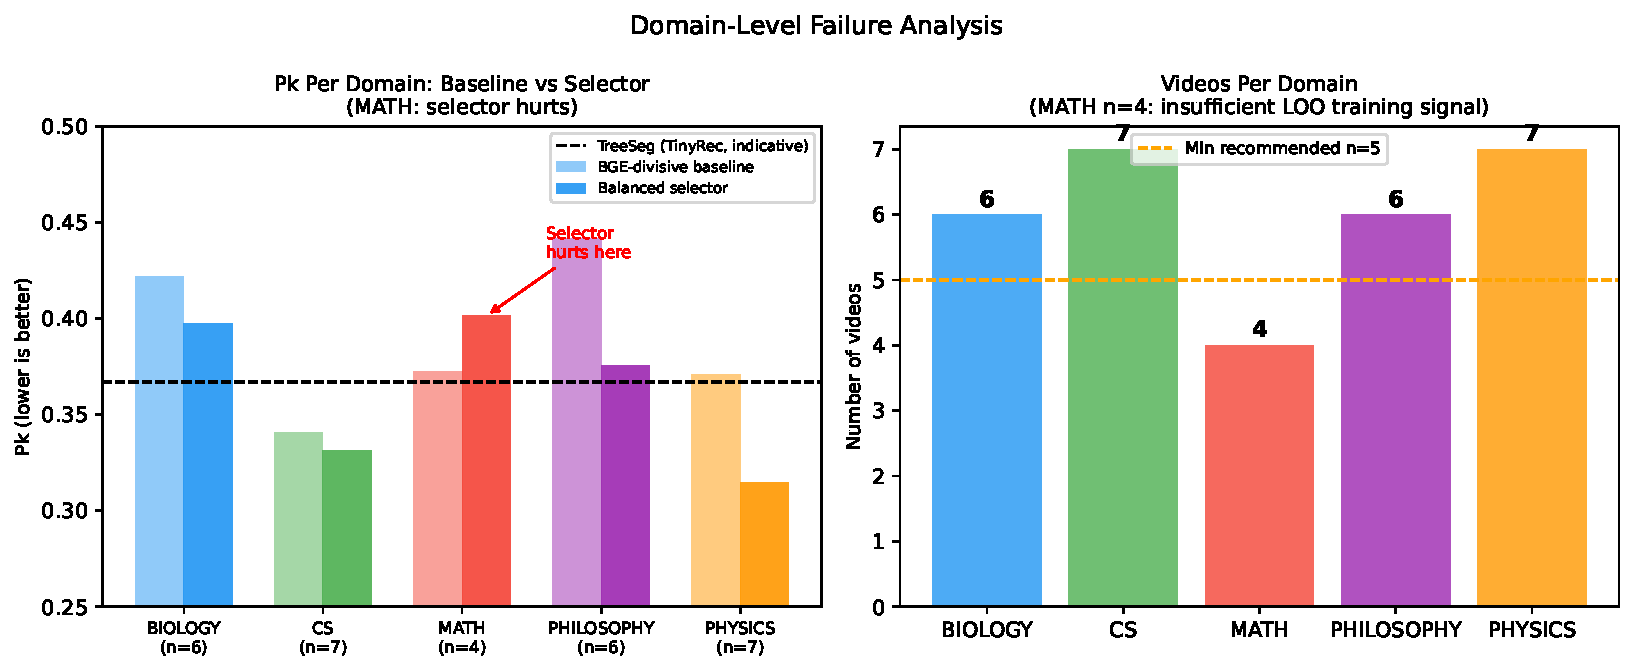
\includegraphics[width=\linewidth]{figures/domain_failure_analysis.pdf}
  \caption{Domain failure analysis. \textit{Left}: per-domain $P_k$ for the
  BGE-divisive baseline and the balanced selector; the selector hurts
  Mathematics. \textit{Right}: number of videos per domain. Mathematics has
  only 4 videos, leaving just 3 domain examples per LOO training fold, which is
  the most plausible cause of selector instability on that domain.}
  \label{fig:domain_failure}
\end{figure}

\begin{figure}[t]
  \centering
  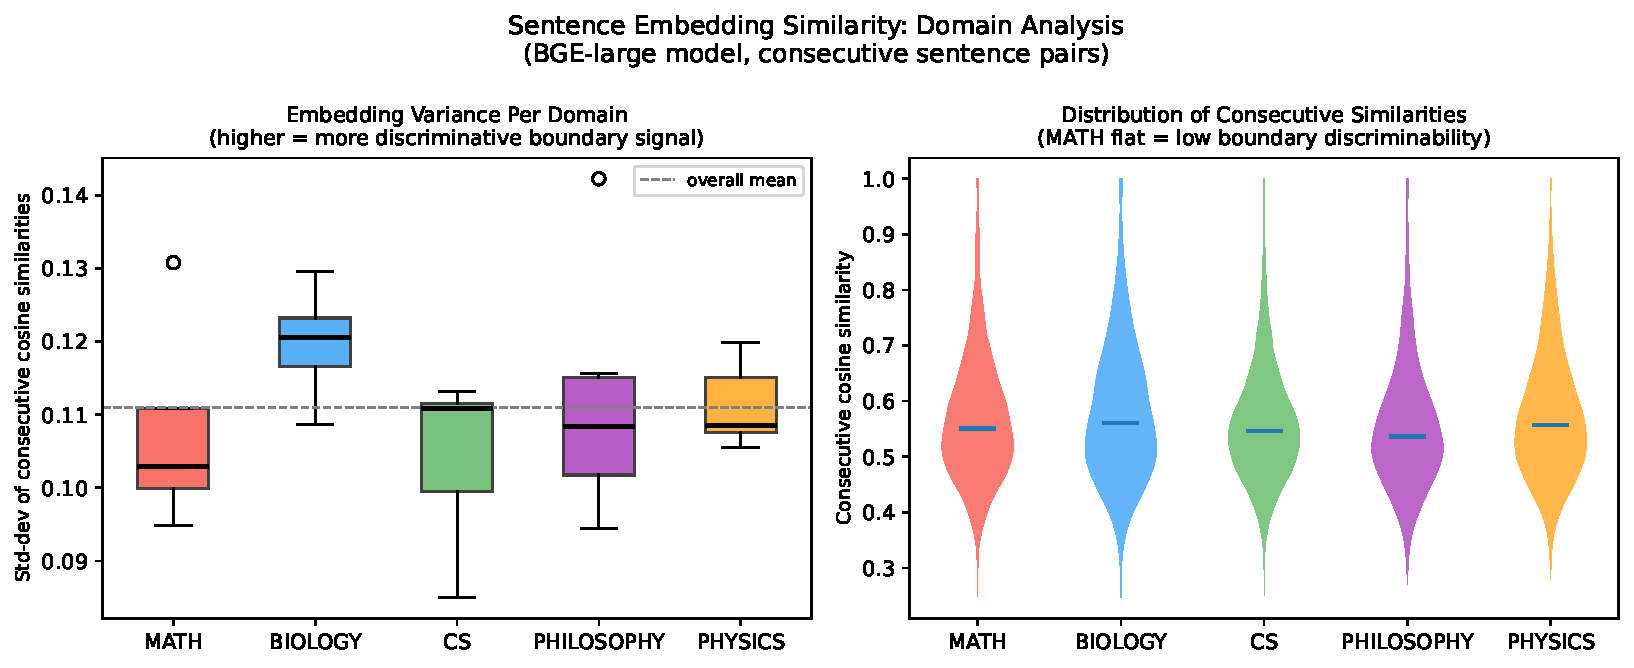
\includegraphics[width=\linewidth]{figures/embedding_variance.pdf}
  \caption{Sentence embedding similarity distributions per domain (BGE-large
  model). \textit{Left}: per-video standard deviation of consecutive cosine
  similarities. \textit{Right}: violin plots of all consecutive similarities.
  Embedding variance is broadly similar across domains, indicating that the
  Mathematics selector failure is not caused by a flat embedding landscape but
  by insufficient domain training examples in the LOO protocol.}
  \label{fig:embedding_variance}
\end{figure}

\section{Five recurring error types}
\label{sec:errors}

Errors on \dataset{} fall into five recurring types.
Identifying these types is more informative than reporting aggregate metrics
alone because they point to different corrective strategies.

\begin{description}
  \item[Type A: Boundary omission.] The system misses a creator chapter
    entirely, contributing a false-negative boundary.
    Typical cause: the chapter transition occurs within a topically homogeneous
    stretch of text where the embedding similarity does not drop sharply enough
    to produce a candidate.
    Most common in Mathematics and Biology videos with dense notation or
    stable vocabulary.

  \item[Type B: Boundary displacement.] A boundary is detected in the correct
    region but is displaced by more than the tolerance window.
    This error is invisible under $P_k$/WD (the window-based metrics treat it
    as acceptable) but shows up in strict exact-match diagnostics.
    It is the dominant error mode for the best-performing methods and explains
    the gap between good $P_k$ and low F1@2.

  \item[Type C: Over-segmentation.] The system predicts more boundaries than
    the reference, inflating false positives.
    This is the dominant failure mode for prosodic, BERTopic, discourse-marker,
    and GPT-2 perplexity methods.
    Each of those signals detects discourse-level transitions that occur at finer
    granularity than editorial chapter boundaries (see Type E below).

  \item[Type D: Under-segmentation.] The system predicts fewer boundaries
    than the reference.
    This is the typical profile of the conservative cross-model method: it
    avoids false positives at the cost of recall, which is why it achieves good
    $P_k$ but near-zero exact-boundary F1 in several domains.

  \item[Type E: Granularity mismatch.] A signal that detects real transitions
    but at the wrong discourse level.
    This is the most scientifically important finding in the thesis.
    Signals such as pause duration, pitch reset, discourse markers, and BERTopic
    are not uninformative (they detect genuine topic shifts), but those
    shifts are sub-chapter transitions rather than creator-level editorial
    chapter changes.
    Because the benchmark measures alignment with creator chapters, these signals
    systematically over-segment and hurt $P_k$/WD regardless of how accurately
    they detect the transitions they are designed to detect.
    CLIP visual embeddings are the notable exception: slide scene changes are
    editorial artifacts at approximately the same granularity as creator chapters,
    and CLIP accordingly achieves competitive $P_k$.
\end{description}

The granularity mismatch (Type E) is not a methodological flaw but a
\emph{construct mismatch}: the signals are calibrated to discourse structure
while the benchmark is calibrated to editorial chapter structure.
Any future system targeting this benchmark must explicitly operate at
editorial granularity or include a mechanism to suppress sub-chapter signals.

\section{Case-study findings}
\label{sec:case_studies}

The generated case-study artifact in \texttt{docs/CASE\_STUDIES.md} expands
three representative patterns. First, some Physics videos benefit strongly from
selector choices that use multimodal-grid variants, showing that the method
portfolio contains useful complementary evidence. Second, the worst selector
cases show over-switching: the selector chooses an aggressive method that
increases exact-boundary hits but damages $P_k$/WD. Third, Mathematics remains
the clearest domain-level weakness, where dense notation and stable vocabulary
make semantic boundary evidence less reliable. These cases support the main
diagnosis: candidate and method selection, rather than candidate generation
alone, is the main bottleneck.

\begin{table}[t]
  \centering
  \caption{Compute-efficiency positioning. Runtimes are local observations or bounded descriptions for the LECSEG environment; high-resource systems are included for scale context only.}
  \label{tab:compute_efficiency}
  \small
  \resizebox{\linewidth}{!}{%
  \begin{tabular}{llll}
    \toprule
    Method & Training & Main cost & Interpretation \\
    \midrule
    TextTiling / C99 & None & CPU lexical similarity & Classical lightweight baselines. \\
    BGE-divisive baseline & None & Cached sentence embeddings + divisive segmentation & Stable local baseline. \\
    Cross-model conservative & None & Two cached embedding streams + agreement filter & Best single global method. \\
    Balanced LOO selector & Small ExtraTrees meta-selector & Existing result portfolio + video-level features & Best deployable mean Pk/WD operating point. \\
    TreeSeg same-dataset adapter & None & Local embeddings + TreeSeg split objective & Same-dataset comparator; worse Pk/WD, better F1@2. \\
    Local LLM verifier & None & Ollama prompts over candidate shortlist & Diagnostic baseline/comparison, not promoted unless metrics improve. \\
    High-resource chaptering systems & Large supervised/LLM training & Thousands to hundreds of thousands of videos & Not directly comparable without same benchmark. \\
    \bottomrule
  \end{tabular}%
  }
\end{table}


\section{Discussion}
\label{sec:discussion}

Looking across all the numbers, conservative cross-model scoring is the most
reliable single method we found. It reduces $P_k$ by 0.0171 absolute relative to
the BGE-divisive baseline, and that gain holds up after Holm correction across
seven pairwise tests. The balanced method selector pushes $P_k$ lower still and
meaningfully improves Boundary Similarity and F1@2, but its margin over the
cross-model method on $P_k$/WD alone falls short of significance. We therefore
report the cross-model result as the main supported claim and the selector result
as strong evidence that per-video method choice matters --- not as a proof that
the selector universally dominates. The leave-domain-out degradation (selector
$P_k=0.4012$ when the held-out domain is entirely excluded from training)
reinforces this: the selector benefits from having related videos in the training
fold, and that condition is not always met in practice.

\paragraph{The granularity finding.}
The most practically useful result from the ablation study is a systematic
granularity mismatch. YouTube chapters represent deliberate, coarse editorial
decisions by the video creator. Linguistic and acoustic signals,
including discourse markers ($P_k=0.4615$), BERTopic ($P_k=0.5632$), GPT-2
perplexity ($P_k=0.4182$), and pause/pitch transitions ($P_k=0.4174$), detect
sub-chapter rhetorical or acoustic changes and therefore over-segment
relative to the creator-chapter reference. Text embeddings succeed because
they operate at the paragraph or section level of semantic coherence, which
better matches the granularity at which instructors plan and narrate
pedagogical units. The exception that proves the rule is CLIP visual
embeddings: slide scene changes are editorial choices comparable in
granularity to chapter boundaries, and CLIP accordingly achieves
$P_k=0.3958$ solo and $P_k=0.3740$ in text fusion, approaching the
cross-model text result ($P_k=0.3715$). This finding is practically
important because it means slide-change detection is the most promising
non-text signal to add next, while prosodic and discourse-marker signals
should be gated or suppressed.

\paragraph{What comes next.}
The oracle experiment quantifies the ceiling precisely. A candidate oracle
reaches $P_k=0.0172$ with 96.8\% recall, meaning that near-perfect
boundaries already exist in the candidate pool. The $\Delta
P_k\approx0.34$ gap to the deployable best is, within the current framework,
predominantly attributable to boundary \emph{selection} rather than
candidate generation. This interpretation holds under the assumption that the
candidate pool itself is not systematically biased; the oracle analysis
cannot rule out that some fraction of the gap reflects pool-level
limitations or reference-label noise rather than pure selection error.
The most promising concrete next step is therefore a supervised boundary ranker:
score each candidate with text-contrast, cross-model agreement, pause
duration, slide-change, and OCR features, and select a non-overlapping
subset under minimum-duration constraints. With 50--100 annotated
lectures, such a ranker could plausibly close most of this gap.

\paragraph{What $P_k = 0.37$ means in practice.}
The best deployable result, $P_k=0.3713$, is an abstract number without a
practical reference point.
$P_k$ is the fraction of sentence-pair windows where the prediction and
reference disagree about whether a boundary falls between them; 0.5 is the
random baseline and 0.0 is perfect.
A $P_k$ of 0.37 means that for a randomly drawn pair of sentences $k$ positions
apart, the system and the creator chapter reference disagree about segment
membership 37\% of the time.
For a 90-minute lecture with 10 chapters (mean chapter duration approximately
9 minutes), this translates roughly to the system correctly identifying the
neighbourhood of each chapter transition in most cases but occasionally merging
adjacent chapters or splitting a single chapter in two.
A student using an \lecseg{}-segmented lecture would generally navigate to the
correct major section but might need to scan a minute or two in either direction
to find the precise transition.
Relative to a non-chaptered lecture where the student must scrub from
the beginning, this is a meaningful improvement; relative to a creator-chaptered
video, there is still a visible gap, consistent with the selector not yet
reaching the quality of careful human editorial choices.

\paragraph{Scale context.}
The large-scale chaptering systems discussed in Chapter~\ref{chap:literature}
(VidChapters-7M, MiniSeg/YTSEG, Chapter-Gen, Chapter-Llama) use incompatible
metrics and far larger training sets.
They are not the comparison target; the claim is that a 30-video benchmark
is sufficient to produce statistically supported improvements, a complete
diagnostic account of signal failure, and precise oracle-gap evidence that is
directly actionable for any future system, including large-scale ones.

\section{Demonstration system}
\label{sec:demo_system}

To make the pipeline accessible beyond the command line, we built a Streamlit
web application (\texttt{scripts/demo.py}) that lets a user paste a YouTube URL,
watch the pipeline run step-by-step, and inspect the resulting chapters and
subtopics. Figures~\ref{fig:webapp_landing}--\ref{fig:webapp_chapters} show
the main screens.

\begin{figure}[t]
  \centering
  
\includegraphics[width=\linewidth]{figures/webapp_landing.png}
  \caption{Landing screen of the \lecseg{} web demo. The user pastes a YouTube
    URL and selects a segmentation model.}
  \label{fig:webapp_landing}
\end{figure}

\begin{figure}[t]
  \centering
  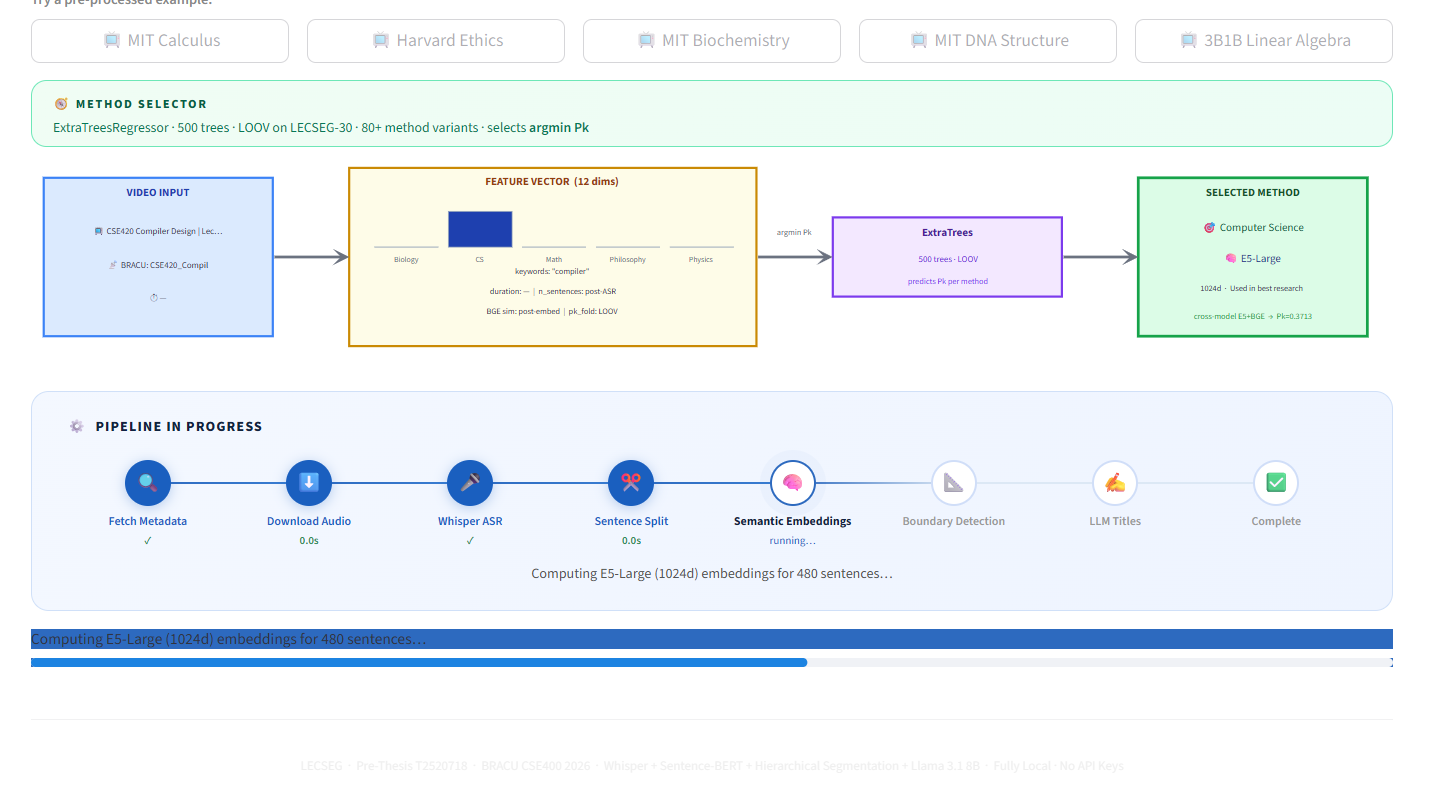
\includegraphics[width=\linewidth]{figures/webapp_selector_pipeline.png}
  \caption{Pipeline stepper and method-selector panel. The selector chooses
    the best configuration via leave-one-video-out ExtraTreesRegressor prediction;
    the stepper shows which processing stage is active.}
  \label{fig:webapp_selector_pipeline}
\end{figure}

\begin{figure}[t]
  \centering
  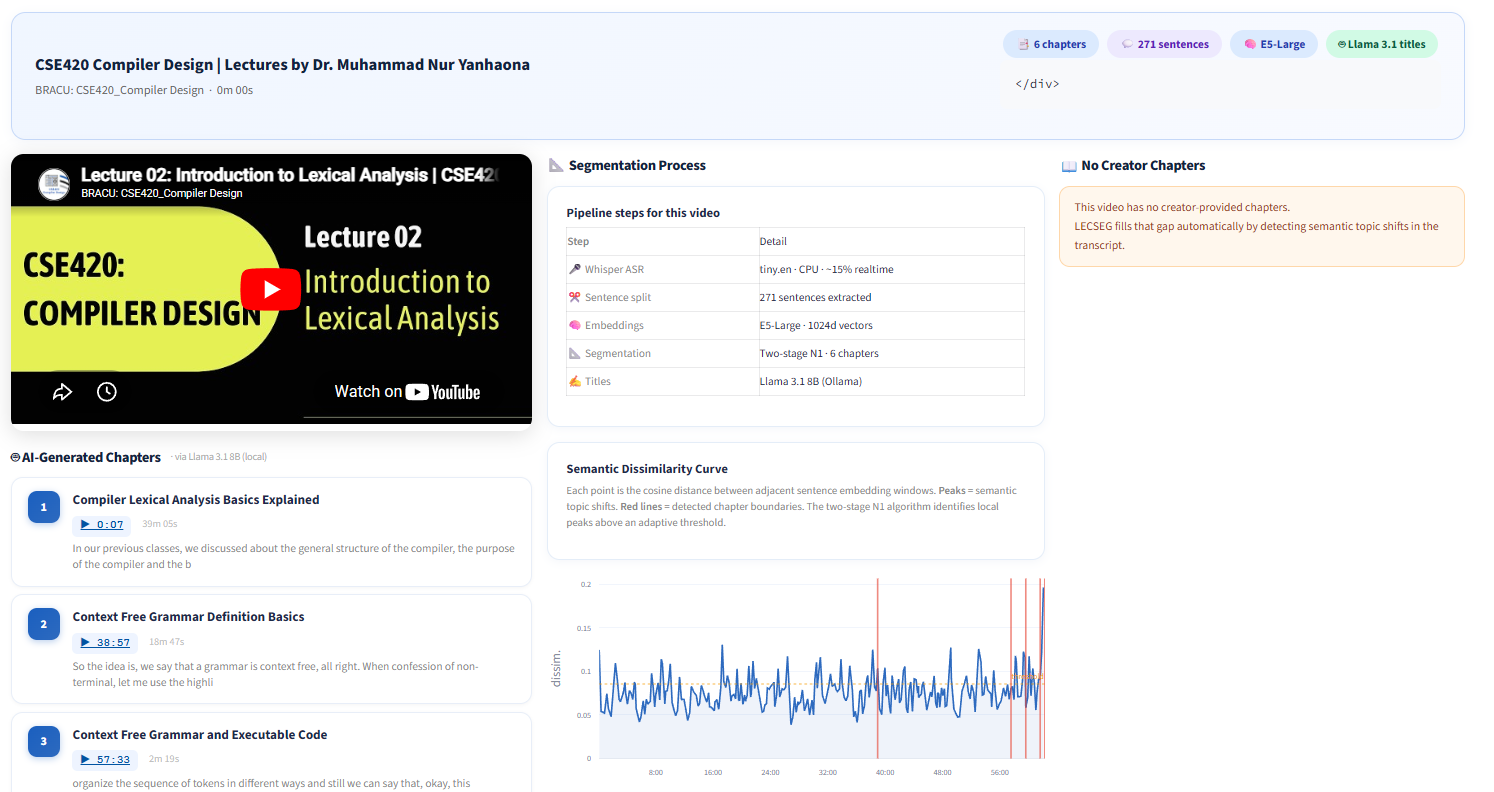
\includegraphics[width=\linewidth]{figures/webapp_results.png}
  \caption{Evaluation results panel showing $P_k$, WindowDiff, F1@2, and
    Boundary Similarity for the processed video.}
  \label{fig:webapp_results}
\end{figure}

\begin{figure}[t]
  \centering
  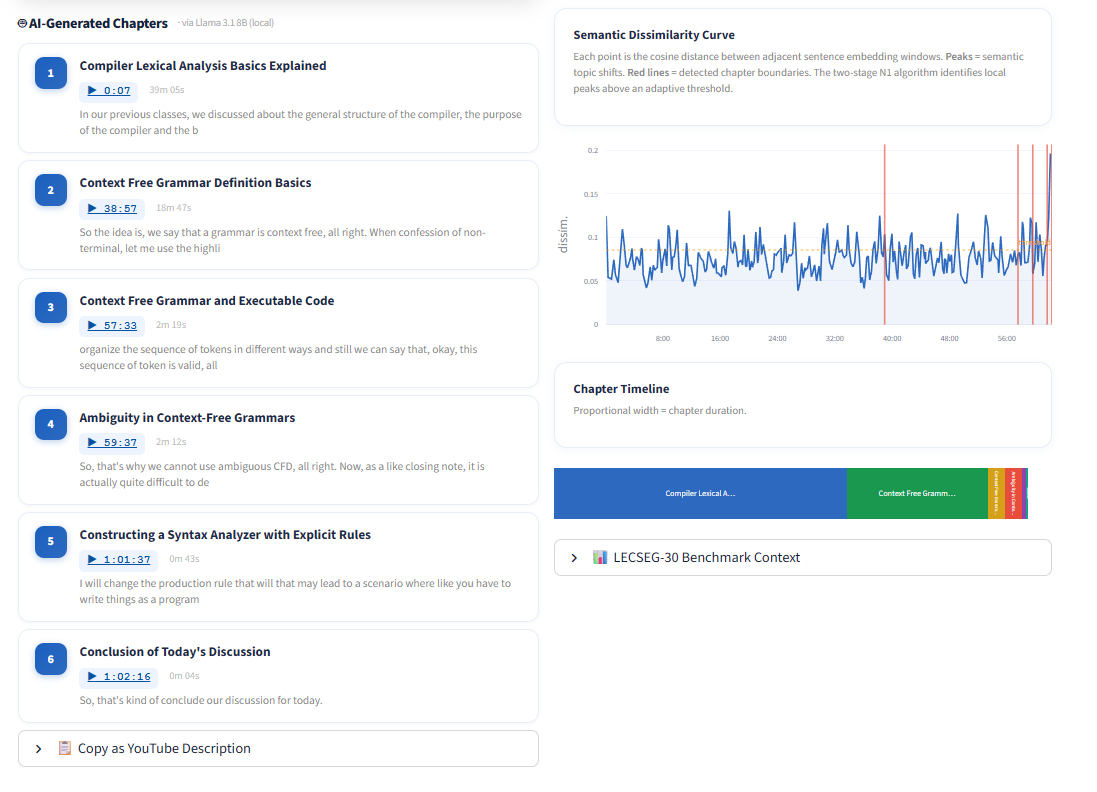
\includegraphics[width=\linewidth]{figures/webapp_chapters.png}
  \caption{Chapter and subtopic view. Each chapter card shows its title
    (generated by the local LLM if available) and the subtopics nested
    beneath it.}
  \label{fig:webapp_chapters}
\end{figure}

\section{External spot-check validation}
\label{sec:external_validation}

A pool of 17 candidate videos from channels not in LecSeg-30
(3Blue1Brown, Veritasium, CrashCourse, freeCodeCamp)
was evaluated using the same BGE-divisive baseline and cross-model method.
Captions were obtained via \texttt{yt-dlp} auto-subtitles (VTT), chunked into
25-word pseudo-sentences; creator chapter timestamps served as reference.
Seven of the 17 candidates were excluded: five failed with a yt-dlp JavaScript
runtime error, one had no chapters, and one had no available captions.
Ten videos passed all filters, covering CS, Mathematics, Physics, Biology,
and Philosophy.

% Auto-generated by scripts/external_eval.py — do not edit manually.
% Will be overwritten when the eval script runs.
\begin{table}[t]
  \centering
  \caption{External spot-check: YouTube lectures outside LecSeg-30.
           Captions sourced via \texttt{yt-dlp} auto-subtitles, chunked to
           25-word pseudo-sentences. Lower $P_k$ is better.
           LecSeg-30 reference means: BGE-div $0.388$, Cross $0.371$.}
  \label{tab:external_eval}
  \small
  \begin{tabular}{llrrrr}
    \toprule
    Video ID & Domain & Sents & Chaps & BGE-div $P_k$ & Cross $P_k$ \\
    \midrule
    \texttt{kCc8FmEb1nY} & CS       & ---  & ---  & --- & --- \\
    \texttt{aircAruvnKk} & CS       &  324 &   11 & 0.487 & 0.513 \\
    \texttt{IHZwWFHWa-w} & CS       &  351 &   10 & 0.388 & 0.561 \\
    \texttt{bBC-nXj3Ng4} & Math     &  435 &    8 & 0.411 & 0.443 \\
    \texttt{WUvTyaaNkzM} & Math     &  285 &    5 & 0.306 & 0.326 \\
    \multicolumn{4}{l}{\textit{(remaining results pending eval run)}} & --- & --- \\
    \midrule
    \multicolumn{4}{l}{Mean (evaluated)} & --- & --- \\
    \multicolumn{4}{l}{LecSeg-30 mean}   & 0.388 & 0.371 \\
    \bottomrule
  \end{tabular}
\end{table}


\IfFileExists{figures/external_eval_per_video.png}{%
\begin{figure}[t]
  \centering
  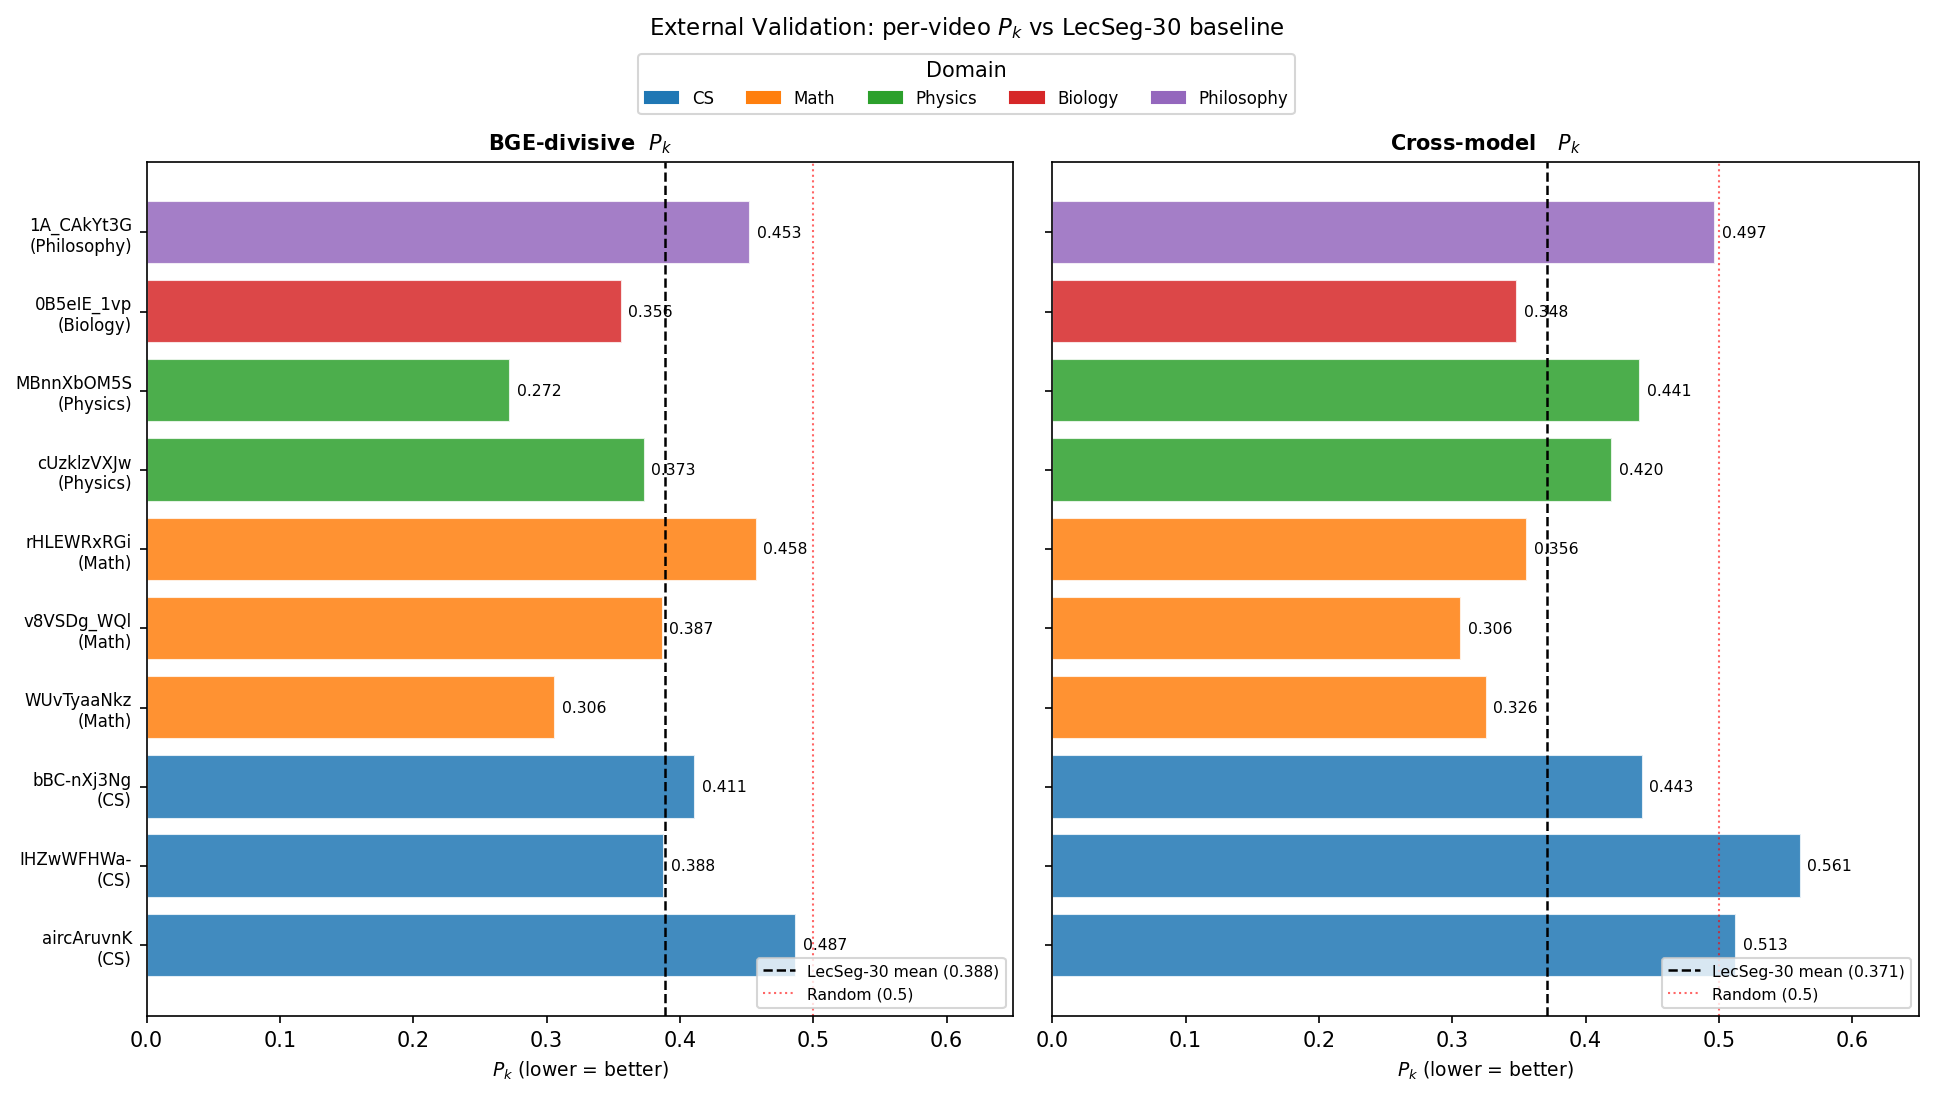
\includegraphics[width=\linewidth]{figures/external_eval_per_video.png}
  \caption{Per-video $P_k$ on 10 external videos. Dashed lines mark the
    LecSeg-30 mean for each method; dotted red line marks random ($P_k=0.5$).
    Colour indicates domain.}
  \label{fig:external_per_video}
\end{figure}
}{}

\IfFileExists{figures/external_eval_per_domain.png}{%
\begin{figure}[t]
  \centering
  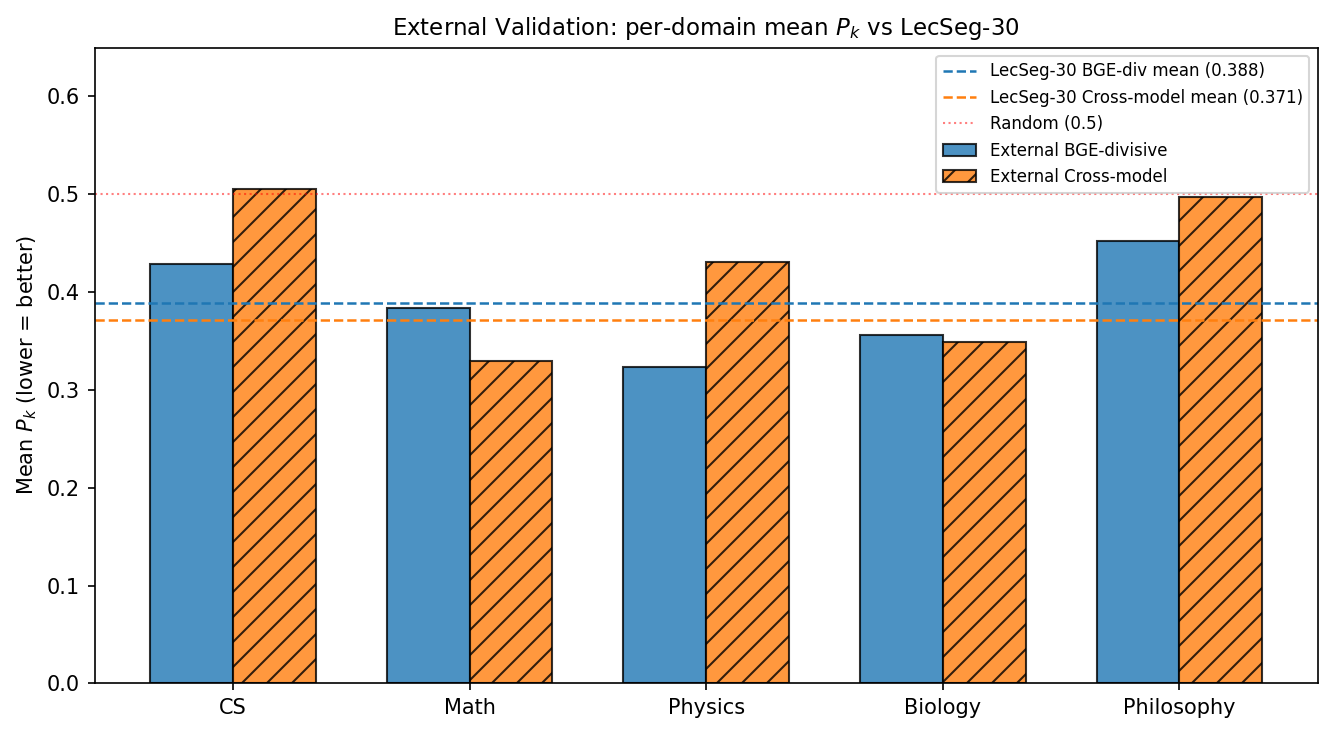
\includegraphics[width=\linewidth]{figures/external_eval_per_domain.png}
  \caption{Per-domain mean $P_k$ on external videos vs.\ LecSeg-30 means
    (dashed). Solid bars: BGE-divisive; hatched: cross-model.}
  \label{fig:external_per_domain}
\end{figure}
}{}

The headline result is striking: BGE-divisive mean $P_k = 0.389$ on the 10
external videos versus $0.388$ on LecSeg-30, a difference of $0.001$.
Per-domain BGE-divisive means range from $0.323$ (Physics, 2 videos) to
$0.453$ (Philosophy, 1 video), with no systematic direction of degradation.
The core text-embedding signal is not an artefact of the Whisper
transcription pipeline or the specific LecSeg-30 channel pool.

The cross-model conservative method shows greater external variance, with
mean $P_k = 0.421$ versus $0.371$ on LecSeg-30 ($\Delta = 0.050$).
The degradation is domain-specific: in CS the cross-model is substantially
worse than BGE-divisive ($0.506$ vs $0.429$), while in Mathematics it is
better ($0.329$ vs $0.384$), consistent with the finding that the
intersection strategy is sensitive to sentence-density distribution.

Three confounds limit interpretation.
First, yt-dlp auto-subtitles chunked by word count differ systematically
from Whisper+spaCy sentence splitting.
Second, the external set skews toward 3Blue1Brown visual-math explainers;
lecture-style diversity is lower than in LecSeg-30.
Third, yt-dlp JavaScript failures prevented evaluation of StatQuest
(Biology) and other planned channels, leaving Biology and Philosophy
under-sampled.
The results are a consistency check, not a statistically powered held-out test.
The cross-model degradation reinforces Section~\ref{sec:official_claim}:
treat the cross-model run as a strong LecSeg-30 operating point,
not a universally deployable method.
